\documentclass[border=12pt]{standalone}
\usepackage{tikz}
\usetikzlibrary{arrows.meta, positioning, calc}
\usepackage{amsmath}
\usepackage{xcolor}

\definecolor{navy}{HTML}{1E2761}
\definecolor{accent}{HTML}{408EC6}
\definecolor{iceblue}{HTML}{CADCFC}
\definecolor{lightbg}{HTML}{F4F6FB}
\definecolor{dgreen}{HTML}{2D8B46}
\definecolor{orange}{HTML}{E07B2E}

\begin{document}
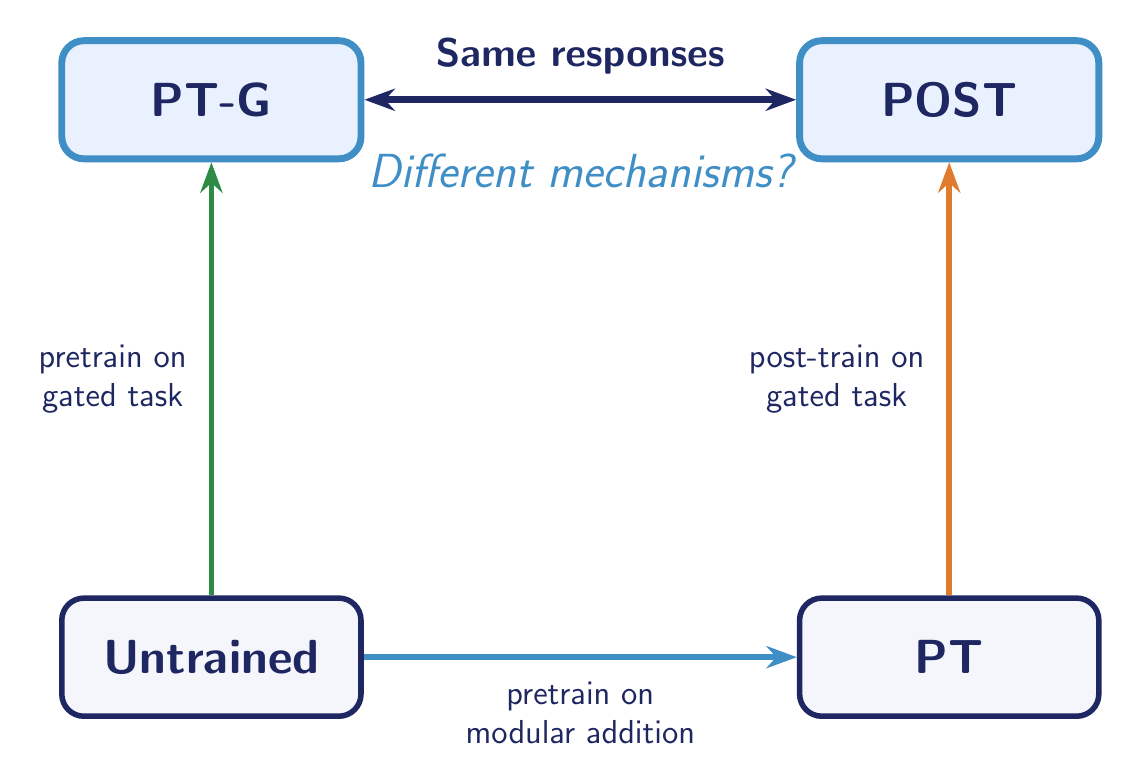
\begin{tikzpicture}[
    node distance=5.5cm and 5.5cm,
    box/.style={
        rectangle, rounded corners=8pt, draw=navy, line width=2pt,
        fill=lightbg, minimum width=3.8cm, minimum height=1.5cm,
        font=\LARGE\bfseries\sffamily, text=navy, align=center
    },
    highlight/.style={
        rectangle, rounded corners=8pt, draw=accent, line width=2.5pt,
        fill=iceblue!40, minimum width=3.8cm, minimum height=1.5cm,
        font=\LARGE\bfseries\sffamily, text=navy, align=center
    },
    lbl/.style={font=\large\sffamily, align=center, text=navy, fill=white, inner sep=4pt, rounded corners=2pt},
]

% Nodes
\node[box] (untrained) {Untrained};
\node[box, right=of untrained] (pt) {PT};
\node[highlight, above=of untrained] (ptg) {PT-G};
\node[highlight, above=of pt] (post) {POST};

% Bottom arrow: Untrained -> PT
\draw[-{Stealth[length=11pt, width=8pt]}, line width=2pt, accent]
    (untrained) -- node[lbl, below=4pt] {pretrain on\\modular addition} (pt);

% Left arrow: Untrained -> PT-G (dark green)
\draw[-{Stealth[length=11pt, width=8pt]}, line width=2pt, dgreen]
    (untrained) -- node[lbl, left=4pt] {pretrain on\\gated task} (ptg);

% Right arrow: PT -> POST (orange)
\draw[-{Stealth[length=11pt, width=8pt]}, line width=2pt, orange]
    (pt) -- node[lbl, left=4pt] {post-train on\\gated task} (post);

% Top double arrow: PT-G <-> POST
\draw[{Stealth[length=11pt, width=8pt]}-{Stealth[length=11pt, width=8pt]}, line width=2.5pt, navy]
    (ptg) -- node[lbl, above=4pt, font=\Large\sffamily\bfseries, text=navy] {Same responses} (post);

% Question below the top arrow
\node[font=\LARGE\itshape\sffamily, text=accent] at ($(ptg)!0.5!(post) + (0,-0.9)$) {Different mechanisms?};

\end{tikzpicture}
\end{document}
